\section{Aufbau}
Zentrales Element des Aufbaus ist der Lock-In-Verstäkrer selbst, verbunden mit einem sogenannten \enquote{Noise Generator}.
All diese fundamentalen Bauelemente sind in einem Gerät mit variablen Nenngrößen verbaut und zum Auslesen an einen Speicher-Oszillator geschlossen.
Um der vollen Funktion des Filters gerecht zu werden, müssen die Elemente in folgender Ordnung miteinander verbunden werden.
\begin{figure}
    \centering
    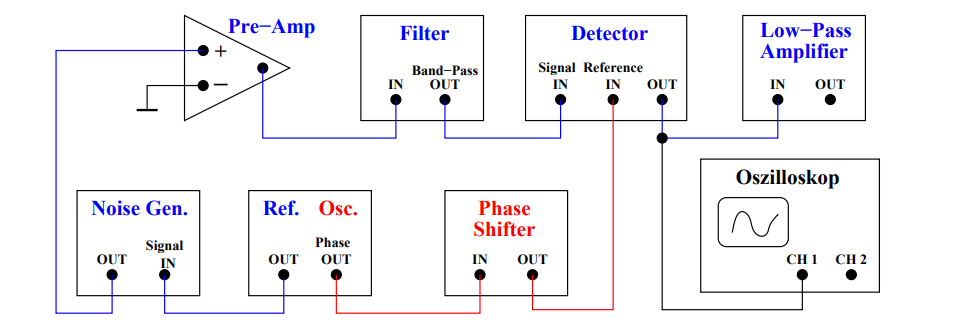
\includegraphics[width=0.8\textwidth]{bilder/plan.png}
    \caption{Schematischer Aufbau eines Lock-In-Verstäkers mit integriertem Noise Generator und Oszilloskop. \cite{skript}} 
    \label{fig:plan}
\end{figure}
Der letztendliche Aufbau ist stark abhängig von den gewählten Einstellungen der einzelnen Filter und der Frequenz der erzeugten Spannung.
\begin{figure}
    \centering
    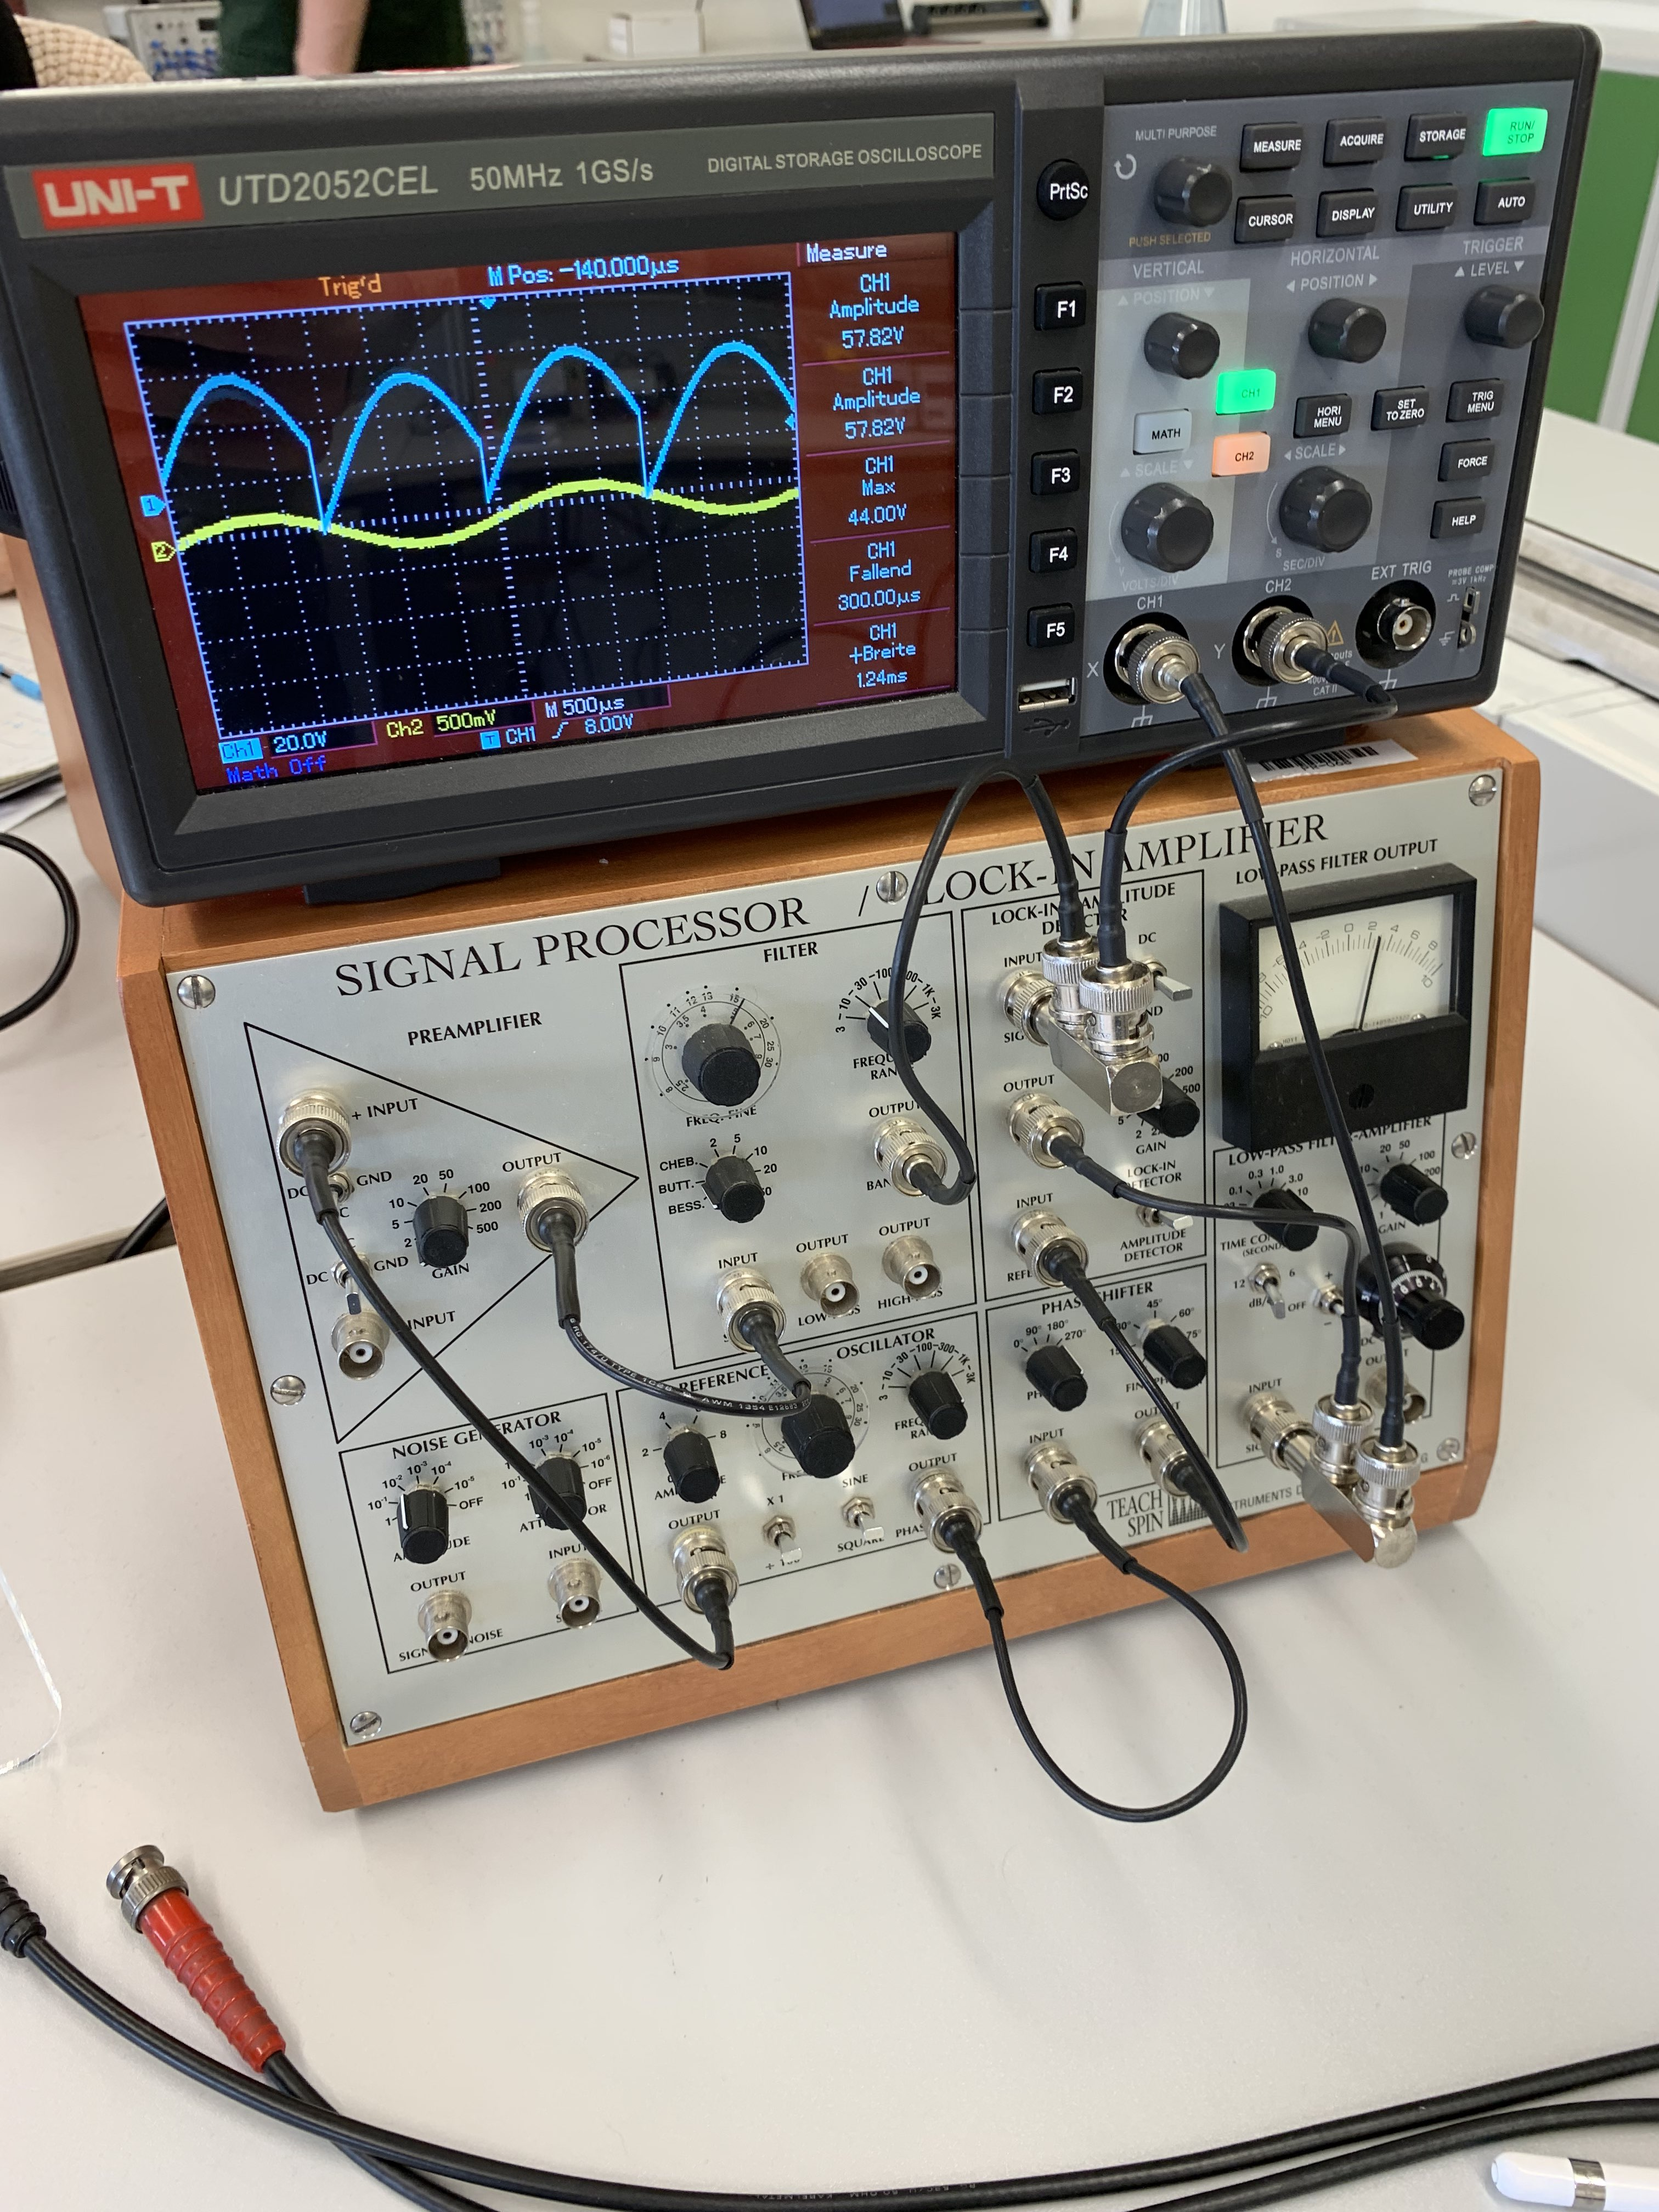
\includegraphics[width=0.4\textwidth]{bilder/RL.png}
    \caption{Finaler Aufbau, bestehend aus Lock-In-Verstäker mit Oszilloskop aber überbrücktem \enquote{Noise Generator}.} 
    \label{fig:RL}
\end{figure}
Diese Art des modularen Aufbaus ermöglicht in der Anwendung eine genaue Untersuchung der einzelnen Elemente und ihre Wechselwirkung.
Der Filter nach dem Preamplifier beinhaltet einen Hoch und Tiefpass was also die Ausgänge verschiedener Versuche stark beeinflusst und folglich auch limitieren kann.
\\
Durch die Einstellungen der Phase am \enquote{Phase Shifter} lässt sich eine Differenz von bis $\SI{360}{\degree}$ in beliebig kleinen Schritten einstellen.
Der integrierte Oszillator kann zwischen einer Sinus - und Rechtecksspannung wechseln wobei die mögliche Frequenz in einem Intervall von $[\SI{3}{\hertz}, \SI{3}{\kilo\hertz}]$ variabel ist.
\\
Das am \enquote{Noise Generator} künstlich erzeugte Rauschen ist in seiner Intensität frei wählbar und kann folglich an den entsprechenden Reglern eingestellt werden.

\section{Durchführung}
Die erste Messreihe beinhaltet den Zusammenhang zwischen Phasendifferenz und der resultierenden Ausgangsspannugn $U_{out}$ mit und ohne Rauschen.
Dafür muss, um ein Rauschen zu vermeiden, vorerst die Schaltung so überbrückt werden, dass der Preamplifier direkt an den Output der 
\enquote{Referenz} angeschlossen ist. In $\SI{45}{\degree}$ Schritten wird nun die Phasendifferenz am \enquote{Phase Schifter} erhöht und die Messwerte am 
Oszilloskop abgelesen. Analog folgt die Messung mit Rauschen wobei der \enquote{Noise Generator} mit in den Schaltkreis integriert ist.
\\
\newline
Um ein künstliches Rauschen durch eine realistische Anwendung zu ersetzen, wird im letzten Teil der Durchführung der Schaltplan so verändert,
dass anstelle des \enquote{Noise Generator} eine LED Lampe mit Photodiode installiert ist. Diese Photodetektorschaltung ist abhängig vom Abstand $r$ zwischen dem Leuchtkörper und dem Detektor
welcher im Verlauf der Messreihe 30 mal verstellt wird. Zentrales Ziel der Messreihe ist die vom Abstand abhängige Amplitude, die am Oszillator abgelsen werden kann.
\begin{figure}
    \centering
    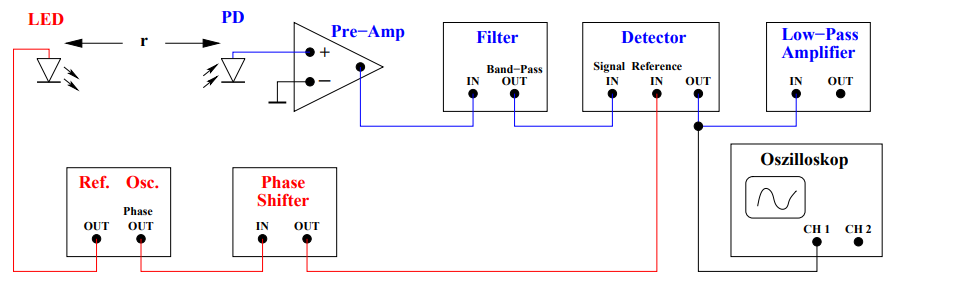
\includegraphics[width=0.6\textwidth]{bilder/licht.png}
    \caption{Schematischer Aufbau des Lock-In-Verstäker mit installiertem Photodetektor. \cite{skript}} 
    \label{fig:licht}
\end{figure}